\section{Closed Innovation}\label{sec:grundlagen-closed}

\paragraph{Ursprung}
Das \textit{Closed Innovation}-Modell ist das vorherrschende Innovationsmodell im 20. Jahrhundert.
Es spiegelt die damalige Wissensumgebung wider.
Unter Wissenschaftlern ist es verpönt ihre Fähigkeiten zu Nutzen um wirtschaftliche Probleme zu lösen.

Um dennoch Innovationen anzutreiben und so den kommerziellen Erfolg zu sichern,
sind Unternehmen gezwungen selbst in \ac{fe} zu investieren.
Da in anderen Unternehmen das notwendige Wissen nicht aufgebaut ist,
müssen Unternehmen innerhalb ihrer \ac{fe}-Organisation das gesamte Spektrum von den Grundlagen bis hin zum fertigen Produkt abdecken.
Voraussetzung hierfür ist die Akquise von talentierten Mitarbeitern.

\todo[inline]{Geschichte etwas ausführlicher? Auch noch Wandlung zu Open Innovation?}

\paragraph{Prinzipien}
Implizit ergeben sich so die Prinzipien der \textit{Closed Innovation} (nach \cite[19]{herzog2011}):
\begin{itemize}
    \item Ein Unternehmen sollte die talentiertesten Mitarbeiter anstellen.
    \item Um von Innovationen zu profitieren, müssen diese innerhalb des Unternehmens den gesamten Innovationsprozess durchlaufen (Vom Entdecken, über das Entwickeln bis hin zur Vermarktung)
    \item Um ein Produkt als erstes auf den Markt zu bringen, muss eine Entdeckung innerhalb des eigenen Unternehmens entstehen.
    \item Durch die Markteinführung als erstes Unternehmen gewinnt es den Wettbewerb
    \item Investiert ein Unternehmen am meisten in \ac{fe}, so entstehen dort die besten Ideen, was wiederum den Wettbewerb gewinnt.
    \item Damit andere Unternehmen nicht von den eigenen Entdeckungen profitieren, gilt es das geistige Eigentum zu schützen.
\end{itemize}

\paragraph{Modell}
Aus diesen Regeln folgt das in \autoref{fig:closedInnovation} dargestellte Modell.
Der gesamte Innovationsprozess spielt sich innerhalb der Grenzen des Unternehmens ab.
Eine Innovation beginnt immer durch eine Idee innerhalb des Unternehmens,
wird durch die firmeneigene \ac{fe}-Abteilung entwickelt
und schließlich auf dem bestehenden Markt des Unternehmens kommerzialisiert.

\begin{figure}[ht!]
    \centering
    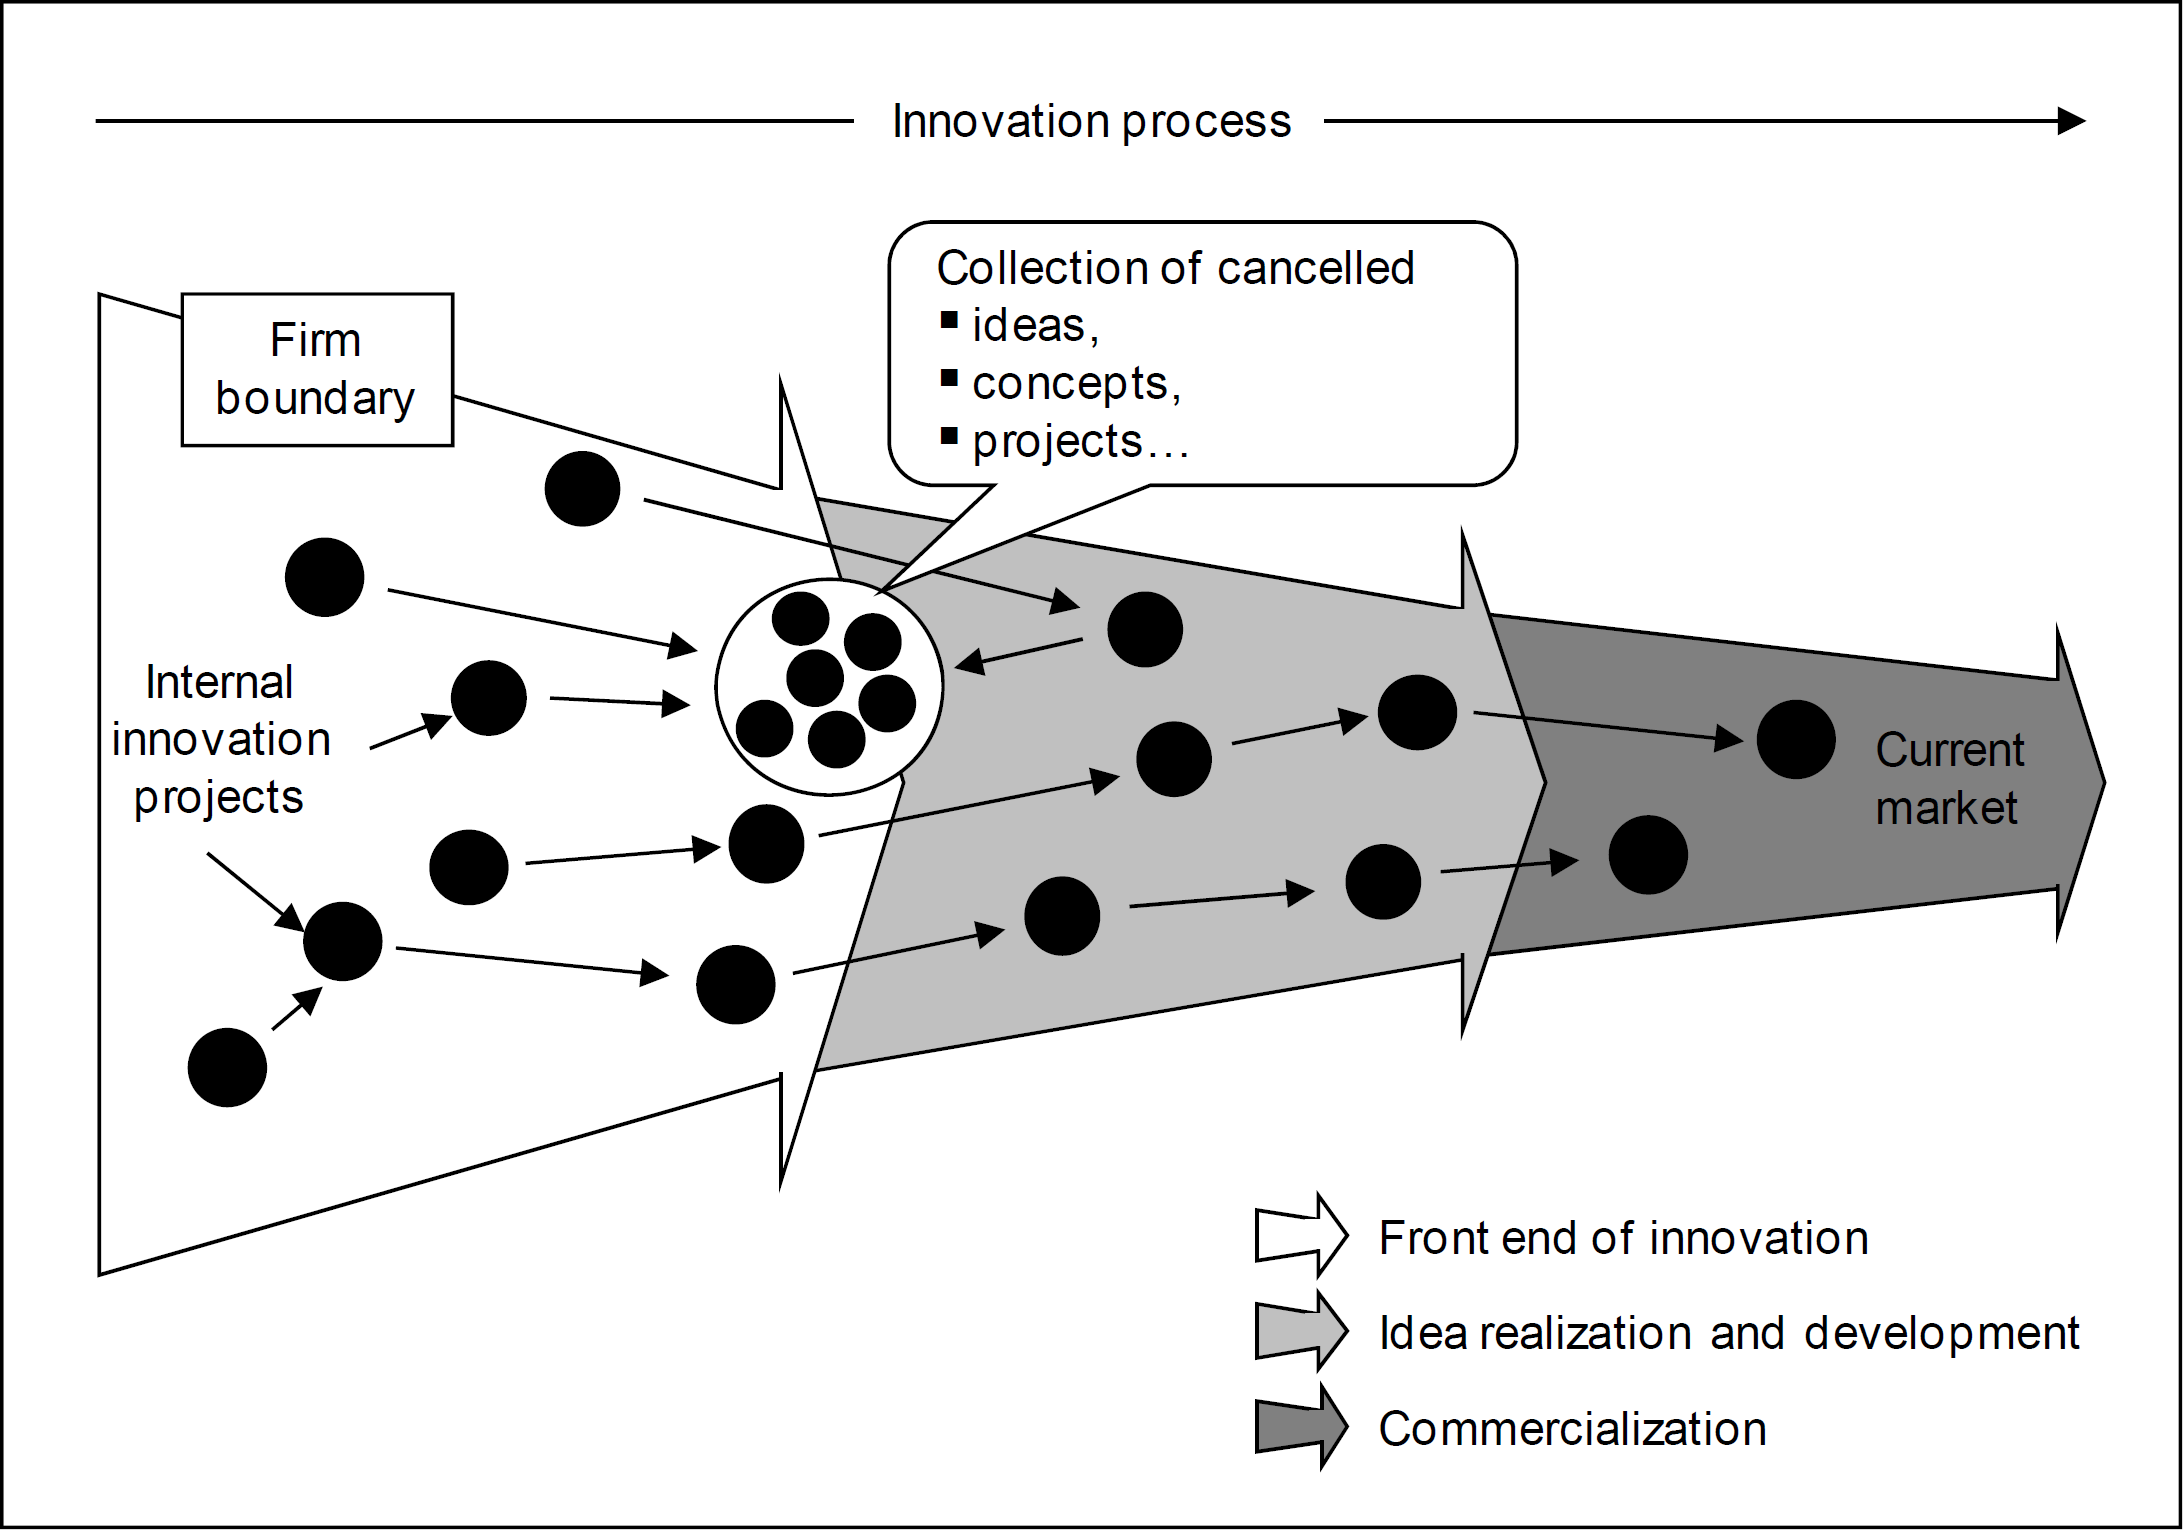
\includegraphics[width=1\textwidth]{ClosedInnovation}
    \caption{Closed Innovation Modell (aus \cite[20]{herzog2011})}
    \label{fig:closedInnovation}
\end{figure}

Selbstverständlich können nicht alle Ideen realisiert werden.
Möglicherweise ist die Ursache hierfür fehlende Ressourcen (Arbeitskraft oder Wissen)
oder es findet sich innerhalb der Unternehmensgrenzen keine vermarktbare Anwendung für eine neue Entdeckung.
Auch werden Ideen gegebenenfalls nicht umgesetzt, da vermutet wird, dass keine Akzeptanz am Markt herrscht.

Abgelehnte Ideen und abgebrochene Projekte werden beispielsweise in Datenbanken gesammelt.
Von dort werden sie wieder aufgegriffen
oder bleiben ein ungenutzter Teil des geistigen Eigentums eines Unternehmens.


